\documentclass[10pt]{beamer}
\usetheme{Malmoe}
\setbeamertemplate{navigation symbols}{}
%\colorlet{beamer@blendedblue}{blue!40!black}
\setbeamertemplate{navigation symbols}{}
\newcommand*\oldmacro{}%
\let\oldmacro\insertshorttitle%
\renewcommand*\insertshorttitle{%
\oldmacro\hfill%
\insertframenumber\,/\,\inserttotalframenumber}

\usepackage{caption}
\usepackage{hyperref}
\usepackage[makeroom]{cancel}
\usepackage{ amssymb }
\usepackage{appendixnumberbeamer}
%\usepackage{tikz-feynman}
\usepackage{graphicx}
\begin{document}

\title{Nationwide: Telematics Assessment Exercises}
\author[Barkeloo]{Jason Barkeloo, PhD}

%\titlegraphic{\includegraphics[width=4cm]{../ATLAS-Logo-Ref-RGB.png}\hspace*{2.75cm}~%
%   \includegraphics[width=4cm]{../uo_logo_green_on_white_2.jpg}
%}

\date{}
\frame{\titlepage}
\frame{\frametitle{Table of Contents}\tableofcontents[hidesubsections]}

\frame{\frametitle{Code location for further fleshed out examples}
\begin{itemize}
\item All code for these exercises can be found via these links as ipython/jupyter notebooks located on my github in addition to attachments sent with the presentation 

\begin{itemize}
\item Part 1: \hyperlink{https://github.com/JTBarkeloo/JupyterNotebooks/blob/master/BarkelooNationwideAssessmentPart1.ipynb}{github: BarkelooNationwideAssessmentPart1.ipynp} 

\item Part 2:  \hyperlink{https://github.com/JTBarkeloo/JupyterNotebooks/blob/master/BarkelooNationwideAssessmentPart2.ipynb}{github: BarkelooNationwideAssessmentPart2.ipynp}
\end{itemize}
\end{itemize}
}

\section{Part 1: GPS Data - Analysis}
\frame{\frametitle{Tasks to be Completed}
Analysis Task:
\begin{itemize}
\item 1: Data Cleaning
\item 2: Setting of hard braking and acceleration thresholds based on the data
\item 3: Trip-by-trip Analysis and Summary
\end{itemize}

Data Set Overview:
\begin{itemize}
\item 9687 rows of 4 variables including:
\begin{itemize}
\item  trip\_id: a trip number identifier 
\item local\_dtm: a datetime timestamp of the event entry
\item latitude: latitudinal coordinate
\item longitude: longitudinal coordinate
\end{itemize}
\end{itemize}
Datasets are loaded into pandas dataframes for further analysis
}

\subsection{Task 1: Data Cleaning}

\frame{\frametitle{Data Cleaning, Gross Features}
\begin{itemize}
\item 3 large unphysical features occur in the dataset (teleportation across the globe for 2-4 seconds)
\item These events are pruned by requiring the latitude and longitude be within $2^{\circ}$ of the median for the data set
\item This includes an area on the order of the state of Ohio
\begin{itemize}
\item Assumption: the sensors are used for checking daily driving habits and not long, rare, road trips
\item No other points are removed under this cut, only these large outliers.  If this assumption is false (i.e., long-haul truck drivers use these), then this would need to be adapted
\end{itemize}
\end{itemize}
\centering
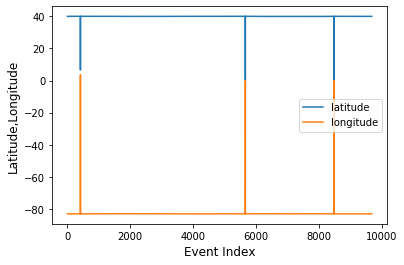
\includegraphics[width=0.5\textwidth]{Images/Image1.png}
}

\frame{\frametitle{Result of Gross Cleaning}
\begin{itemize}
\item  The median cut above leaves the longitude and latitude plots in a reasonable state
\item Some very fast jumps are still seen which are coincident, typically, with a change in trip\_id (GPS drift while off) 
\item Can calculate distance between any two points using the geodesic distance making use of geopy package
\item From this data and corresponding timestamps in local\_dtm plots of the speed $s = \frac{\Delta\text{Position}}{\Delta\text{Time}}$ and acceleration $a = \frac{\Delta\text{Speed}}{\Delta\text{Time}}$ can be made
\end{itemize}
\centering
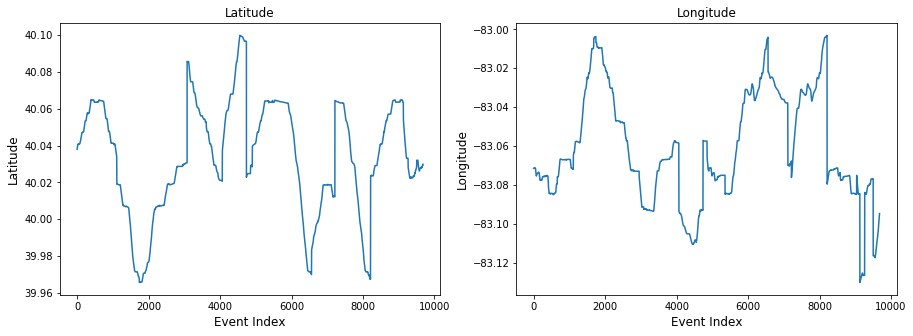
\includegraphics[width=1.\textwidth]{Images/Image2.png}
}

\frame{\frametitle{Further Cleaning - $\Delta$Position, $\Delta$Time, Speed, Acceleration}
\centering
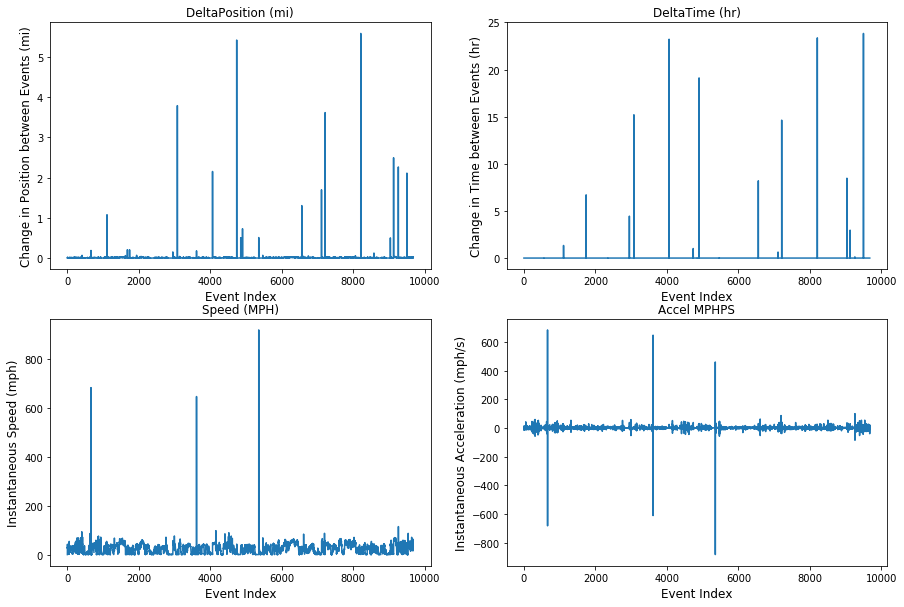
\includegraphics[width=1.\textwidth]{Images/Image3.png}
}

\frame{\frametitle{More Features to be Cleaned}
\begin{itemize}
\item From $\Delta$Position, $\Delta$Time we see the large number of drifts which account for the GPS drift from trip differences
\item 15 events: These jumps will not be an issue when analyzing trip-by-trip as the change in position starts from the first point of the trip
\item Speed and Acceleration plots show an additional 3 further unphysical events.  These are resultant from small GPS errors for a few seconds and need to be cleaned
\item Another issue comes when $\Delta$Time between events is 0 i.e., if the frequency drops below 1Hz and the readings are taken within a second.
\begin{itemize}
\item 24 events: A 0th order approach is taken to these points and only the first point is kept.  An alternative would be averaging the latitude/longitude for the points.  This would be a change within the same second and as such would not have much of an effect that is not then averaged out in the acceleration
\end{itemize}
\end{itemize}
}

\frame{\frametitle{Gross Feature Cleaning - Speed and Acceleration Plots}
\begin{itemize}
\item The clear erroneous events in the speed and acceleration curves are cleaned by looking at large speed values ($>100$mph) using coincidence points that also correspond to accelerations that are not possible by the majority of cars ($>30$mph/s)
\begin{itemize}
\item After these cleaning steps have occured most of the obvious points have been removed
\item Remaining oscillations are closer to the scale of the data
\item To smooth out itinerant spikes and general noise, a rolling average using a 3 event window is used on speed and acceleration
\end{itemize}
\end{itemize}

\centering
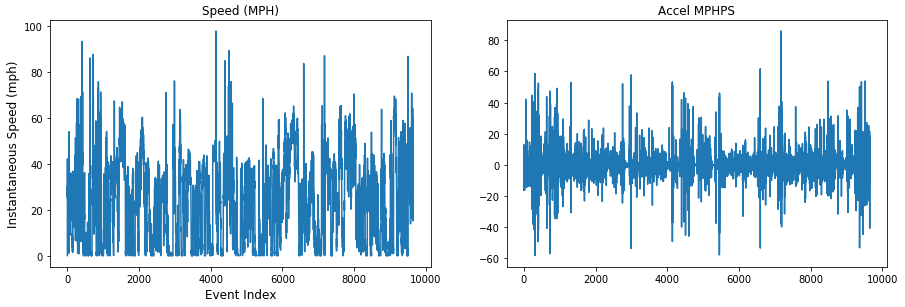
\includegraphics[width=.8\textwidth]{Images/Image4a.png}
}

\frame{\frametitle{Speed, After Cleaning}
\begin{itemize}
\item Window size 3 average helps filter noise, still keeps large fast features
\end{itemize}
\centering
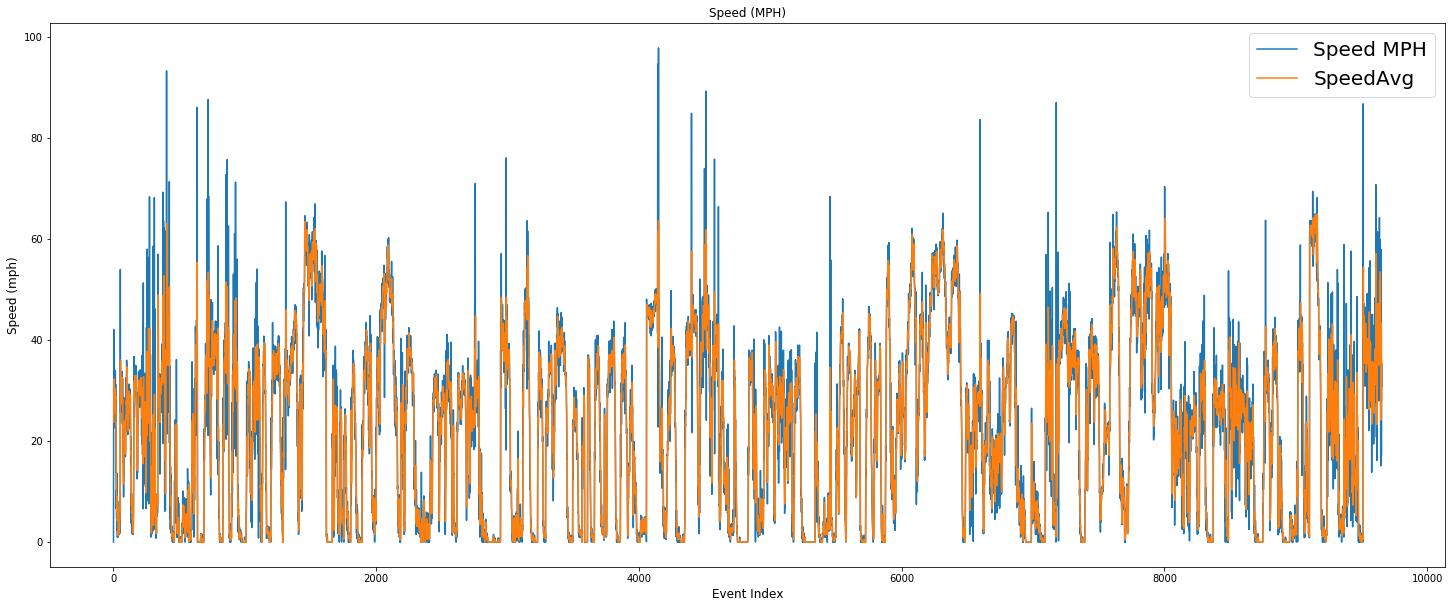
\includegraphics[width=1.\textwidth]{Images/Image5.png}
}

\frame{\frametitle{Acceleration, After Cleaning}
\begin{itemize}
\item Accel: Directly calculated from change in speed values
\item AccelAvg: Calculated using the change in the rolling average of speed values
\item AccelAvg3: Calculated using the rolling average of acceleration values
\end{itemize}
AccelAvg3 is the least spiking and as such will be used as the acceleration value going forward for threshold setting
\centering
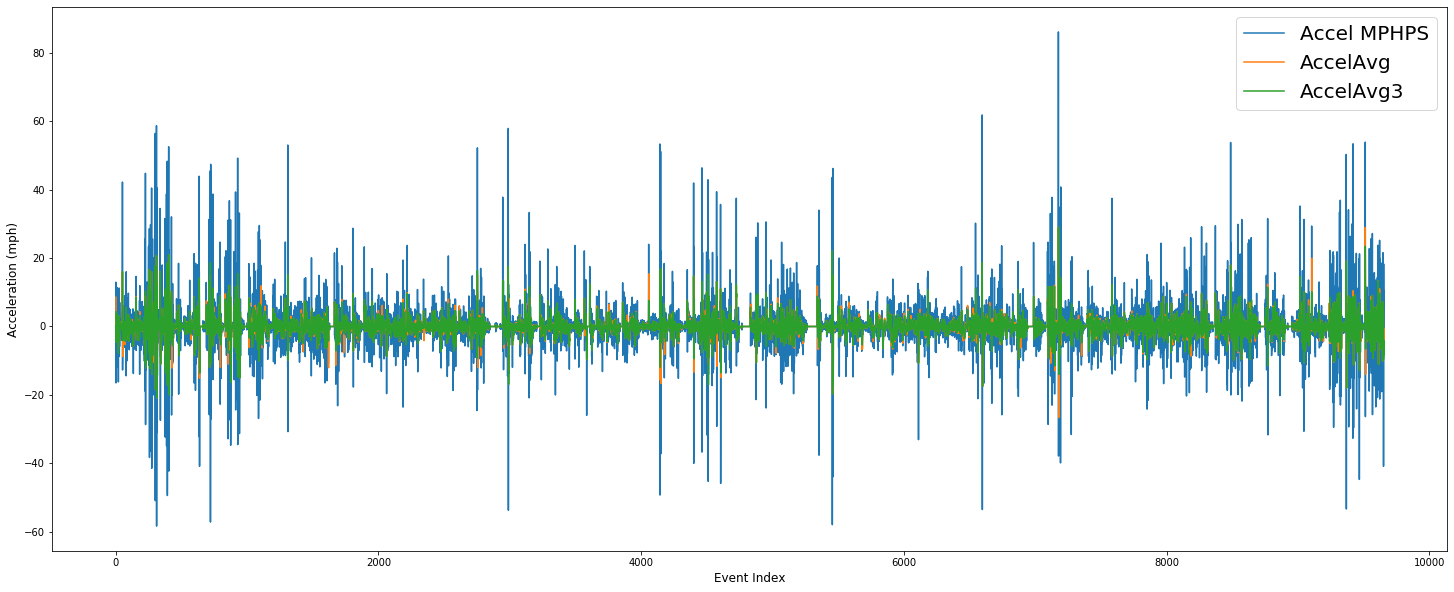
\includegraphics[width=1.\textwidth]{Images/Image6.png}
}

\subsection{Task 2: Threshold Setting}
\frame{\frametitle{Task 2: Setting Hard Event Thresholds}
Hard Braking/Acceleration Events
\begin{itemize}
\item Assume average acceleration is roughly normal (mean = 0.07, std= 2.71) to consider positive and negative accelerations half-normal distributions $\rightarrow \sigma=\bar{a}\sqrt{\pi/2}$
\begin{itemize}
\item Positive Acceleration-  mean: 1.71 mph/s  std: 2.14 mph/s
\item Negative Acceleration-  mean: -1.62 mph/s   std: -2.03 mph/s
\end{itemize}
\item Thresholds set for both distributions at 2 standard deviations away from the mean
\begin{itemize}
\item Hard Acceleration: $>$5.99 mph/s
\item Hard Braking: $<$-5.68 mph/s
\end{itemize}
\end{itemize}
\centering
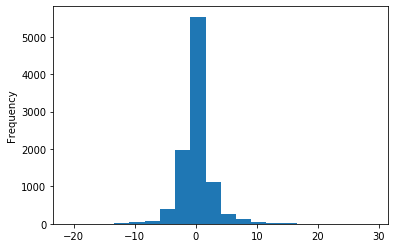
\includegraphics[width=0.5\textwidth]{Images/Image8.png}
}

\frame{\frametitle{Hard Event and Idle Time Definition}
Hard Events
\begin{itemize}
\item Number of peaks beyond the threshold using the rolling average acceleration
\item Using rolling average and looking for local peaks in the acceleration landscape limits multicounting of the same `Event'
\end{itemize}
Idle Time Definition
\begin{itemize}
\item Total time spent with rolling average speed $<$1mph
\end{itemize}
}

\subsection{Task 3: Trip-by-Trip Summaries}
\frame{\frametitle{Task 3: Trip-by-Trip Summaries}
Trip-by-Trip Speed and Acceleration Plots
\begin{itemize}
\item Blue are raw values and orange are rolling averages
\end{itemize}
\centering
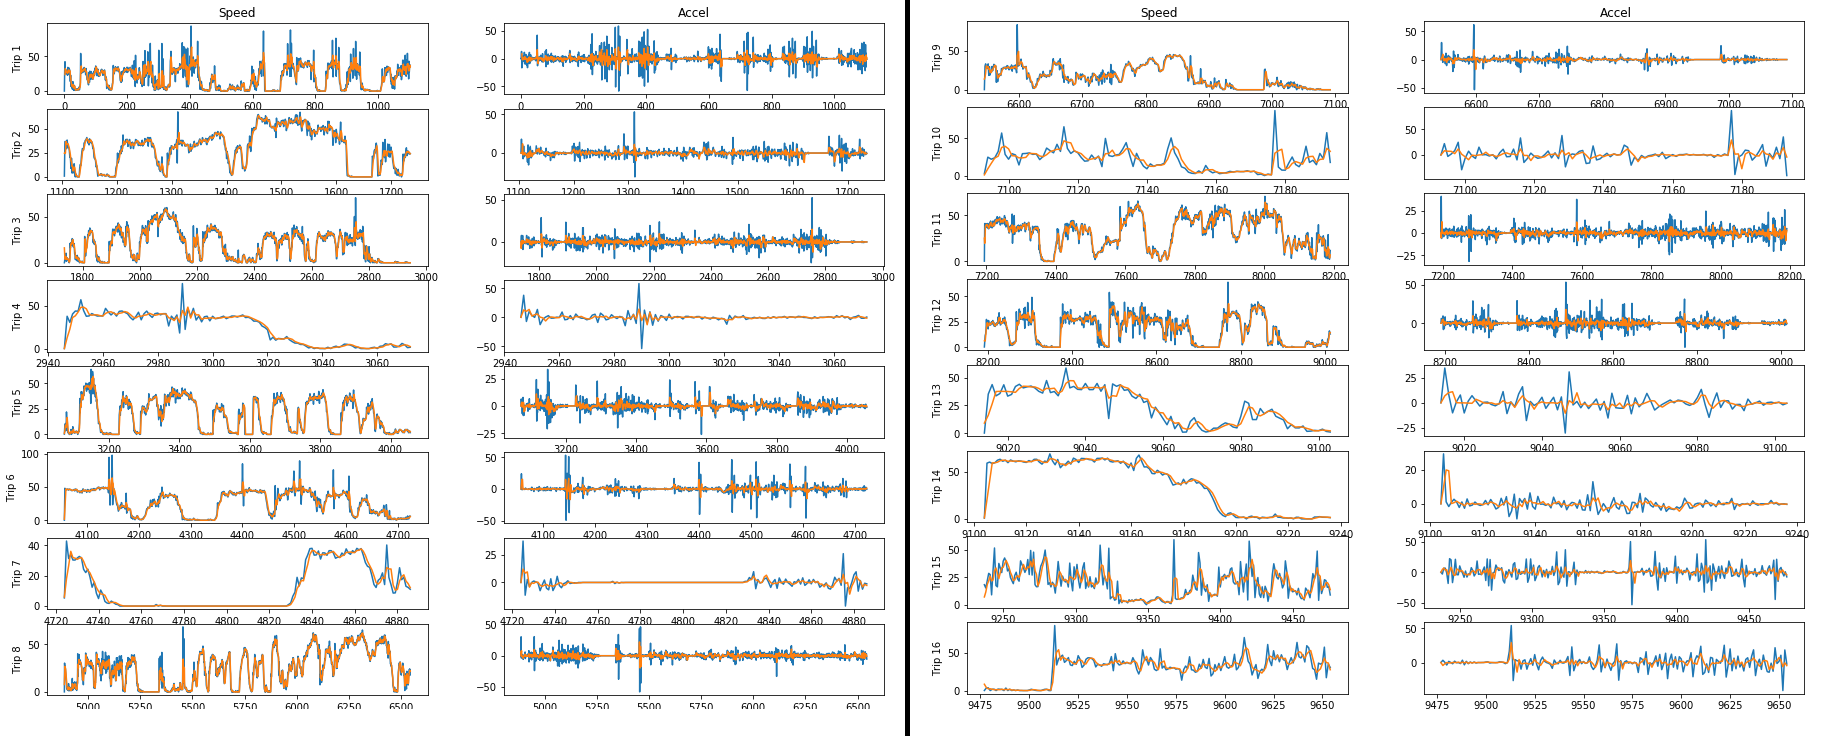
\includegraphics[width=1.\textwidth]{Images/Image7.png}
}



\frame{\frametitle{Trip Summaries}
\centering
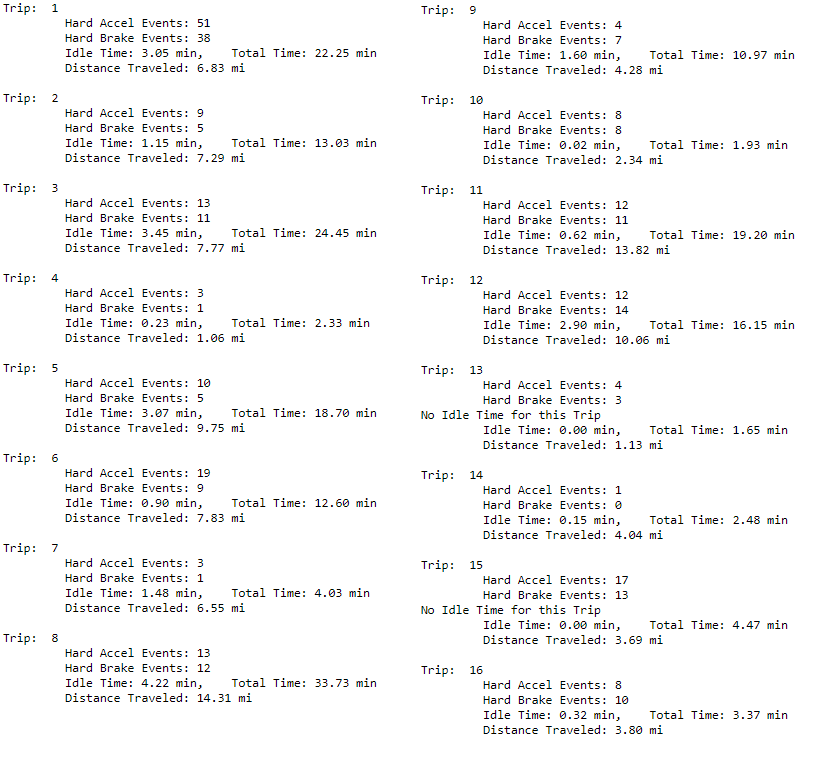
\includegraphics[width=0.78\textwidth]{Images/Image9.png}
}


%%%%%%%%%%%%%%%%%%%%%%%%%%%%%%%%%%%%%%%%%%%%%%%%%%%%%%%%%%%%%%%%%
\section{Part 2: Modeling}
\frame{\frametitle{Part 2: Modeling - Simulated Dataset Overview}
Summary of 30,000 vehicles 1Hz telematics datasets
\begin{itemize}
\item Vehicle - Effectively an index on the data
\item Days - Number of days data was collected (365 for all)
\item Distance - Total number of miles vehicle was driven during data collection
\item HardBrakes - Number of hard braking events detected
\item HardAccelerations - Number of hard acceleration events detected
\item NightTime\_Pct - Percentage of total miles driven at night
\item VehicleType - str description of type of vehicle
\item Loss - Indicator if vehicle has been in a collision
\end{itemize}
Want to build a model that will optimize recognition of Loss events using these values
%\centering
%\includegraphics[width=0.7\textwidth]{../../ThesisImages/backgrounds.png}
}

\subsection{Task 4: Statistical Significance Between Vehicle Types}

\frame{\frametitle{Task 4: Statistical Significance of Loss Between Vehicle Types}
\begin{itemize}
\item  Assuming the Loss populations are sampled from a binomial distribution with probablity LossPerType/TotalPerType, then a z-test can be conducted to determine if the null hypothesis (distributions are sampled from the same distribution) can be rejected
\item For a significance $\alpha = 0.05$ a z-value greater than the critical value of $z_c=1.64$ implies rejection of the null hypothesis
\item For repeated tests the Look-Elsewhere effect/multi-comparison problem should also be taken into consideration, changing the critical value $z_c = 2.64$
\end{itemize}

\centering
\begin{columns}
\begin{column}{0.5\textwidth}
$z   = \frac{p_1 - p_2}{\sqrt{p (1-p)(1/n_1 + 1/n_2)}}$ \\
\end{column}
\begin{column}{0.5\textwidth}
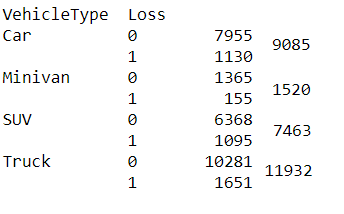
\includegraphics[width=0.8\textwidth]{Images/Image10.png}
\end{column}
\end{columns}
}

\frame{\frametitle{Statistical Significance Between Vehicle Types}
The conclusions to be drawn depend on how liberal the definition of statistical significance being used is \\ 
The use of p$<$0.05 is somewhat arbitrary but is what will be used here as it is a standard choice of convention
\begin{itemize}
\item \fbox{z value for Car and Minivan: 2.48} 
\item z value for Car and SUV: 4.19 
\item z value for Car and Truck: 2.96 
\item z value for Minivan and SUV: 4.59 
\item z value for Minivan and Truck: 3.92 
\item \fbox{z value for SUV and Truck: 1.62} 
\end{itemize}
The null hypothesis cannot be rejected for the combination of Cars and Minivans and the combination of SUVs and Trucks \\
The implication then is that there are 2 distributions being sampled for these simulated events. This matches intuition as Trucks/SUVs exist in a cargo-loading domain while Cars/Minivans are what parents may gravitate toward% which would describe the necessity of multiple distributions
}



\subsection{Task 5: Hard Brake and Acceleration Importance }

\frame{\frametitle{Task 5: Are Hard Brakes and Accelerations equally important in predicting risk?}
Basic stats about the HardBrakes and HardAccelerations per Loss event and comparing to NoLoss events can give us insight on the separation power of these variables

Loss Events:
\begin{itemize}
\item HardBrakes - mean: 170.24,  median: 98
\item HardAccelerations - mean: 138.25, median: 68
\end{itemize}

NoLoss Events:
\begin{itemize}
\item HardBrakes - mean: 167.44,  median: 98
\item HardAccelerations - mean: 104.53, median: 56
\end{itemize}

Looking at the median values of these Loss events leads to the conclusion that Loss events have more HardAccelerations but a similar number of HardBrakes to NoLoss events \\
This matches my intuition that a larger number of HardAccelerations is an indicator of more aggressive driving
%\centering
%\includegraphics[width=0.7\textwidth]{../../ThesisImages/backgrounds.png}
}


%%%%%%%%%%%%%%%%%%%%%%%%%%%%%%%%%%%%%%%%%%%%%%%%%%%%%%%%%%%%%%%%%%
\subsection{Model Building}

\frame{\frametitle{Model Building}
Primarily employing densely connected feed forward neural networks for event classification was chosen as it is the machine learning model I have most experience with for binary classification
\begin{itemize}
\item 1 input layer with all potentially useful features (Distance, HardBrakes, HardAccelerations, NightTime\_Pct, VehicleType)
\item 2 hidden layers with 20 nodes each
\item Each hidden layer has 20\% dropout to avoid overfitting
\item 1 output layer
\item Activation Function: ReLU on input nodes and hidden layers with Sigmoid on the output layer
\begin{itemize}
\item ReLU is efficient and reduces vanishing gradient problems as the gradient is linear throughout the positive regime
\item Sigmoid gives an output that we can interpret as a probability distribution
\end{itemize}
\item Optimization Function: Adam (Adaptive moment estimation)
\item Loss Function: Binary Cross-entropy
\end{itemize}
A training (64\%)/testing(16\%)/validation(16\%) random set split was done to help ensure unbiased results
%\centering
%\includegraphics[width=0.7\textwidth]{../../ThesisImages/backgrounds.png}
}

\frame{\frametitle{Naive Approach Neural Network}
\begin{itemize}
\item Naively we could train a neural network on the data classes as given
\item With enough separation power i.e., variables distinct enough in each class, this can be used for event classification
\item This is not the case for this dataset, only a few variables inputs with a lot of distribution overlap
\item This would then be expected to fail with a total accuracy that trends toward the class representation of the majority class, which is seen here
\end{itemize}
\begin{columns}
\begin{column}{0.5\textwidth}
\includegraphics[width=0.9\textwidth]{Images/Image11.png}
\end{column}
\begin{column}{0.5\textwidth}
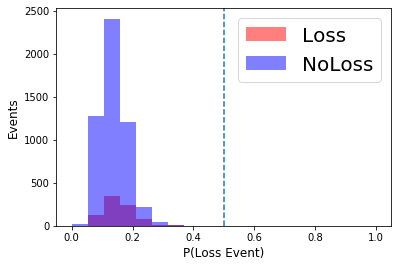
\includegraphics[width=0.9\textwidth]{Images/Image12.png}
\end{column}
\end{columns}
}

\frame{\frametitle{Neural Network with ADASYN Upsampling}
\begin{itemize}
\item In order to ensure equal class representation the minority class is upscaled using synthetic data created using Adaptive Synthetic (ADASYN) over-sampling
\item ADASYN generates synthetic data using weighted distributions for different minority class examples, generating more data on harder to learn events
\item ADASYN shifts the decision boundary toward harder to learn events 
\end{itemize}
\begin{columns}
\begin{column}{0.5\textwidth}
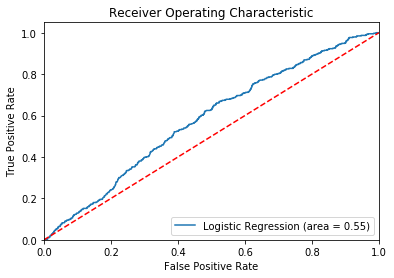
\includegraphics[width=0.9\textwidth]{Images/Image13.png}
\end{column}
\begin{column}{0.5\textwidth}
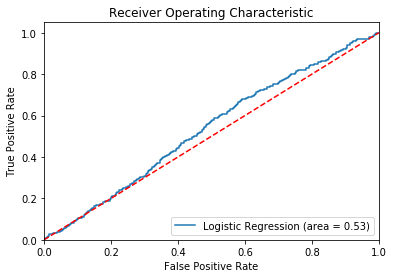
\includegraphics[width=0.9\textwidth]{Images/Image14.png}
\end{column}
\end{columns}
Loss Events P(Loss Event): mean: 0.535, std: 0.094 \\
NoLoss Events P(LossEvent): mean: 0.503, std: 0.092 \\
Loss Event Accuracy: 61.2\%
}

\frame{\frametitle{Neural Network with SMOTE Upsampling}
\begin{itemize}
\item Another network was created and trained using Synthetic Minority Oversampling Technique (SMOTE) over-sampling with similar results
\item SMOTE generates synthetic data that is similar to, but not exactly like the minority class, using a nearest-neighbors approach and fills in space between neighbors
\end{itemize}
\begin{columns}
\begin{column}{0.5\textwidth}
\includegraphics[width=0.9\textwidth]{Images/Image15.png}
\end{column}
\begin{column}{0.5\textwidth}
\includegraphics[width=0.9\textwidth]{Images/Image16.png}
\end{column}
\end{columns}
Loss Events P(Loss Event): mean: 0.510, std: 0.096 \\
NoLoss Events P(LossEvent): mean: 0.480, std: 0.097 \\
Loss Event Accuracy: 55.7\%
}

\frame{\frametitle{Model Comments}
\begin{itemize}
\item  Neural networks have been created and trained on a limited set of input variable with success in determination of Loss events
\item The addition of further independent input variables would help the separation of the neural network greatly
\item A bifurcation of the distributions is starting to occur with the ADASYN network, more input variables and events is likely to cause a major splitting of the distribution into likely Loss events and likely NoLoss events \\
%\item ADASYN over-sampling focuses on the decision boundary which leads to large flucuations in the validation accuracy
\item Boosted decision tree (BDT) models were also employed in the Jupyter notebook to slightly different ends
\end{itemize}
}

%\frame{\frametitle{}
%}

\section{Data Set Enhancement}

\subsection{Additional Research Questions}
\frame{\frametitle{Additional Research Questions: 1}
Can Multiple Loss Models be Useful Based on Driver Class i.e., Rural Vs. Urban Drivers?
\begin{itemize}
\item Rural and Urban drivers face different landscapes of challenges on their daily travels
\item Requirement: GPS definition of urban environments
\item Expect longer distance/trip for rural drivers while urban drivers have more stop-and-go traffic 
\item Larger Distances and a larger amount of HardAccelerations are both positvely correlated with loss this seems to be an interesting intersection of these correlations
\end{itemize}
\centering
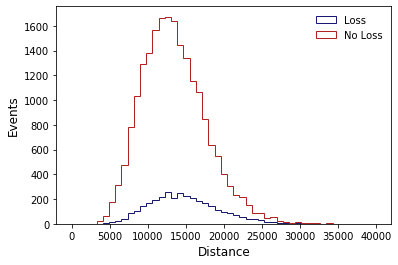
\includegraphics[width=0.4\textwidth]{Images/image18.png}
}

\frame{\frametitle{Additional Research Questions: 2}
Can Adherance to Speed Limit be Calculated and Used in Analysis of Loss?
\begin{itemize}
\item GPS Coordinates can be traced back to roads that have known speed limits (i.e., Apple Maps shows expected speed limits while navigating)
\item An advanced analysis on a percentage of time above some threshold around the speed limit could point towards more high-risk behavior
\item Including this additional variable in loss models could prove beneficial for risk modeling
\end{itemize}
%\centering
%\includegraphics[width=0.7\textwidth]{../../ThesisImages/backgrounds.png}
}

\frame{\frametitle{Additional Research Questions: 3}
Does Average Acceleration During Bearing Change Provide Benefit in Modeling Risk?
\begin{itemize}
\item Events with large accelerations have been used throughout my analysis within this assessment: HardBreaks and HardAccelerations
\item Hard Turning i.e. a large acceleration as measured by an accelerometer when GPS bearing changes by $75-115^{\circ}$
\item HardTurns could prove to be another advantageous metric for evaluating the driving habits of an individual and could be corrected in a similar way as HardBrakes/Accelerations
\end{itemize}
%\centering
%\includegraphics[width=0.7\textwidth]{../../ThesisImages/backgrounds.png}
}

\subsection{Additional Dataset Attributes}
\frame{\frametitle{Additional Dataset Attributes}
Additional attributes to add to the dataset for model improvement
\begin{itemize}
\item Driver Age - Age is historically one of the major factors impacting insurance rates (i.e., Age$\geq$ 25 leads to a lower rate) if this is true it should be beneficial as a discriminating variable 
\item Driver Sex - Another historical risk factor for risk that would be both interesting to analze and I have always been curious about
\item Driving Record: Number of at-fault incidents/Violations -  A driver with 0 to 1 at fault incident, especially with a long driving record (correlation to Age), is surely less likely to cause additional Loss Events
\item Driver Home Location: Address/Zip Code - Leads towards a start of my urban/rural question on a smaller scale but will give first order estimations of the day-to-day driving experience.  This also can lead towards accounting for weather induced Loss
\item Driver Credit Score - As a stand-in for financial responsibility and fitness credit scores could have a small effect on the model as a surrogate for overall responsibility
\end{itemize}
%\centering
%\includegraphics[width=0.7\textwidth]{../../ThesisImages/backgrounds.png}
}

\subsection{Estimate of Sample Size for Additional Research}
\frame{\frametitle{Estimate Sample Size Needed for Additional Research}
All of these estimates are done assuming access to the additional discriminating variables about the driver I have requested
\begin{itemize}
\item Question 1 (Rural/Urban Loss):  Equal sized data sets (50k each, Rural/Urban Drivers) with the additional variables should be sufficient for results to measure the ability to calculate differential loss probability between the two classes
\item Question 2 (Speed Limit Adherance): Further analysis could be done on every existing dataset to include checks to the posted speed limits and amount of time spend significantly above those speed limits.  The nontrivial part is integration of GPS data to speed limit data which can be done after sensors have been collected
\end{itemize}

%\centering
%\includegraphics[width=0.7\textwidth]{../../ThesisImages/backgrounds.png}
}

\frame{\frametitle{Estimate Sample Size Needed for Additional Research}
\begin{itemize}
\item Question 3 (HardTurn Accelerations):  A dataset of 100-200k trips would be a sufficient minimum to start setting a threshold for the acceleration occuring during turns.  The GPS sensors would need to have an internal accelerometer to get more precise instantaneous information during the turn than could be reasonably expected from GPS coordinates alone.  A dataset of this many trips would include perhaps millions turns even though a small fraction of those would be HardTurn accelerations
\end{itemize}
While more data is always better, datasets slightly larger or on the order of what was given for this example with additional discriminating variables assumed to be correlated with Loss prediction will allow a machine learning algorithm much more room to improve and isolate the phase space of high-risk drivers
}

%\frame{\frametitle{Conclusion}
%\begin{itemize}
%\item Orthogonal validation/control regions are in development
%\end{itemize}
%}


%%%%%%%%%%%%%%%%%%%%%%%%%%%%%%%%%%%%%%%%%%%%%%%%%%%%%%%%%%%%%%%%
%%%%%%%%%%%%%%%%%%%%%%%%%%%%%%%%%%%%%%%%%%%%%%%%%%%%%%%%%%%%%%%% 	
%\appendix
%\section{Backup}
%\frame{\frametitle{Backup}
%}
\end{document}

%36.070
